%%%%%%%%%%%%%%%%%%%%%%%%%%%%%%%%%%%%%%%%%%%%%%%%%%%%%%%%%%%%%%%%%%%%%%%%%%%%%
%
%  System        : 
%  Module        : 
%  Object Name   : $RCSfile$
%  Revision      : $Revision$
%  Date          : $Date$
%  Author        : $Author$
%  Created By    : Robert Heller
%  Created       : Sat Apr 15 10:37:45 2023
%  Last Modified : <230416.1413>
%
%  Description 
%
%  Notes
%
%  History
% 
%%%%%%%%%%%%%%%%%%%%%%%%%%%%%%%%%%%%%%%%%%%%%%%%%%%%%%%%%%%%%%%%%%%%%%%%%%%%%
%
%    Copyright (C) 2023  Robert Heller D/B/A Deepwoods Software
%			51 Locke Hill Road
%			Wendell, MA 01379-9728
%
%    This program is free software; you can redistribute it and/or modify
%    it under the terms of the GNU General Public License as published by
%    the Free Software Foundation; either version 2 of the License, or
%    (at your option) any later version.
%
%    This program is distributed in the hope that it will be useful,
%    but WITHOUT ANY WARRANTY; without even the implied warranty of
%    MERCHANTABILITY or FITNESS FOR A PARTICULAR PURPOSE.  See the
%    GNU General Public License for more details.
%
%    You should have received a copy of the GNU General Public License
%    along with this program; if not, write to the Free Software
%    Foundation, Inc., 675 Mass Ave, Cambridge, MA 02139, USA.
%
% 
%
%%%%%%%%%%%%%%%%%%%%%%%%%%%%%%%%%%%%%%%%%%%%%%%%%%%%%%%%%%%%%%%%%%%%%%%%%%%%%

\subsection{Yard Throat with track selector}
\label{sect-appl:yardthroat}

\begin{figure}[hbpt]\begin{centering}%
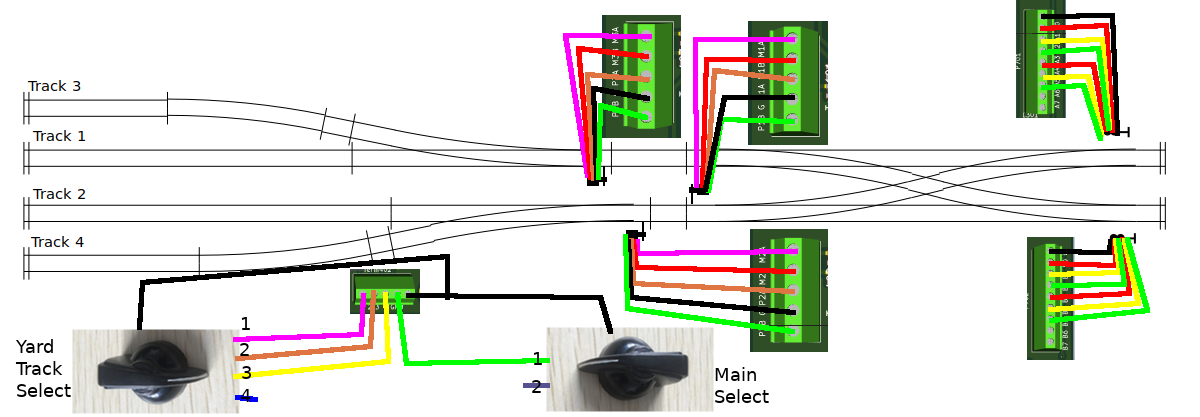
\includegraphics[width=5in]{YardThroat_TrackSelector.png}
\caption{Yard throat with yard ladders and selectors.}
\label{fig:YardThroatTrackSelector}
\end{centering}\end{figure}

This is the entrance to a yard from a double track main line with a scissors 
type crossover and a simple yard ladder.  There are two selector switches, one 
to select the main track and one to select the yard track.  There are a pair 
of signals at the yard entrance, one for each main line track.  These are 3 
over 3 signals.  The basic wiring is shown in 
Figure~\ref{fig:YardThroatTrackSelector}. We will use three turnout drivers 
(the Stall Motor daughter board is shown, but any of the daughter 
boards could be used), 12 of the signal lamp driver outputs, and all four of 
the button inputs.

We will start by configuring the user name and description of the node in User 
Info tab.  When we have done this will will be able to find the node by 
looking for the name.  

Next, we will move onto the Board Configuration tab and give names to the 
Turnout and Points we will be using.

Then we will move onto the button inputs.  The rotary switches total 6 
positions, but we can get by with only 4 inputs, by leaving one position of 
each switch unconnected.  This works because we get extra state information in 
the form of ``none of the above'' -- when all three of buttons 1, 2, and 3 are 
``off'', yard track 4 is selected and when button 4 is off, main track 2 is 
selected.

The logic for the yard track selection is:

\begin{verbatim}
if button1 is on then
  track 1 selected
else if button2 is on then
  track 2 selected
else if button3 is on then
  track 3 selected
else
  track 4 selected
\end{verbatim}

and the logic for the main track selection is:

\begin{verbatim}
if button4 is on then
  main track 1 selected
else
  main track 2 selected
\end{verbatim}

The logic for the scissors crossover is:

\begin{verbatim}
if ( track 1 selected OR track 3 selected) AND 
   main track 1 selected then
  NORMAL
else if ( track 1 selected OR track 3 selected) AND 
        main track 2 selected then
  REVERSE
else if ( track 2 selected OR track 4 selected) AND 
        main track 1 selected then
  REVERSE
else if ( track 2 selected OR track 4 selected) AND 
        main track 2 selected then
  NORMAL
\end{verbatim}

This may \textit{look} formidable, but we can simplify things using a
``trick'' -- a kind of ``wired or'', by using a common event id to represent a
common routing for the odd and even yard tracks. This simplifies things to

\begin{verbatim}
if common odd tracks AND main track 1 selected then
  NORMAL
else if common even tracks AND main track 2 selected then
  NORMAL
else if common even tracks AND main track 1 selected then
  REVERSE
else if common odd tracks AND main track 2 selected then
  REVERSE
\end{verbatim}

We will start by allocating four successive logic elements, setting first
three to have a Group Function of Group and the last to have a Group Function
of Last (Single). We will set the descriptions of these logic elements to
``Track 1'', ``Track 2'', ``Track 3'', and ``Track 4''. The first three will
have a Logic function of V1 only, and the last to null $=>$ true. We will copy
the button event ids from Buttons 1 through 3 to the V1 events of the first
three logic elements: the ``Button Pushed'' event ids to the ``set variable
true'' event ids and the ``Button Released`'' event ids to the ``set variable
false'' event ids.

We will set action 1 of each of these logic elements to an action of Immediate 
if True, and copy the event ids as follows:

\begin{itemize}
\item Track 1: to Turnout 3's Normal.
\item Track 2: to Turnout 2's Normal.
\item Track 3: to Turnout 3's Reverse.
\item Track 4: to Turnout 2's Reverse.
\end{itemize}

Next we will allocate four more Logic elements. Name these ``Main Track 1
Odd'', ``Main Track 2 Even'', ``Main Track 1 Even'', and ``Main Track 2 Odd''.
Set the Group Function of all of them to Last (Single). Set the Logic Function
of all four to V1 and V2. Copy Button 4's ``Button Pushed'', and ``Button
Released'' event to the V1 ``Set variable true'' of both ``Main Track 1''
logics' ``Set variable true'' (Button Pushed) and ``Set variable false''
(Button Released). Copy Button 4's ``Button Pushed'', and ``Button Released''
event to the V1 ``Set variable true'' of both ``Main Track 2'' logics' ``Set
variable true'' (Button Released) and ``Set variable false'' (Button Pushed).
For the variable V2 events we will copy their events to to the Action 2 events
of the Track 1 through Track 4 logics. The odd logics V2 true to get copied to
the odd tracks and their V2 false get copied to the even tracks. And it is
swapped for the even logics. We will end up with two event ids:

\begin{itemize}
\item Odd tracks true / Even tracks false Event: Action 2 events of Track 1 
and Track 3 and the V2 true of ``Main Track 1 Odd'' and ``Main Track 2 Odd'' 
and the V2 false of ``Main Track 1 Even'' and ``Main Track 2 Even''.
\item Even tracks true / Odd tracks false Event: Action 2 events of Track 2 
and Track 4 and the V2 true of ``Main Track 1 Even'' and ``Main Track 2 Even'' 
and the V2 false of ``Main Track 1 Odd'' and ``Main Track 2 Odd''.
\end{itemize}

\begin{figure}[hbpt]\begin{centering}%
\includegraphics[width=5in]{YardThroat_YardSelect.pdf}
\caption{Yard Throat Selection Event Id graph. Color Key: Button Inputs in yellow, Logic elements in cyan, and Turnouts in green.}
\label{fig:YardThroatYardSelect}
\end{centering}\end{figure}

A graph of the Yard Throat Selection Event Id ``flow'' is shown in 
Figure~\ref{fig:YardThroatYardSelect}.  This may look a but intimidating, but 
each ``edge'' (line with an arrow) represents a producer / consumer.  When 
multiple edges land at a given spot, the edges all represent the \textit{same} 
event id.  It is easiest to copy the destination (consumer) Event ID to each 
of the various producers. 
